\begin{center}
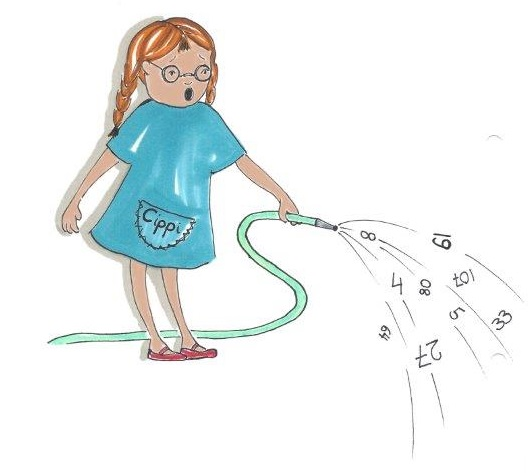
\includegraphics[width=0.6\textwidth]{content/3/chapter6/images/2.png}\\
Cippi在浇花
\end{center}

协程是可以在保持其状态的同时,暂停和恢复其执行的函数。

\begin{tcolorbox}[breakable,enhanced jigsaw,colback=red!5!white,colframe=red!75!black,title={挑战:理解协程}]
	
对我来说,理解协程是一个相当大的挑战,所以强烈建议不要按顺序阅读本章后续的章节。在第一次阅读中跳过“6.1.3 框架”和“6.1.5 工作流”部分,直接阅读“7.2 Future的变化”,“7.3 生成器的修改和泛化”和“7.4 不同的工作流”。阅读、研究和使用所提供的示例,应该会让您对协程的细节和工作流有初步和直观的了解。
	
\end{tcolorbox}

这一节中提到的新思想,其实相当古老。协程这个术语是由\href{https://en.wikipedia.org/wiki/Melvin_Conway}{Melvin Conway}创建,他在1963年关于编译器构造的出版物中使用了这个词。\href{https://en.wikipedia.org/wiki/Donald_Knuth}{Donald Knuth}将程序称为协程的一种特殊情况。有时,需要一段时间来接受这样的设定。

\begin{center}
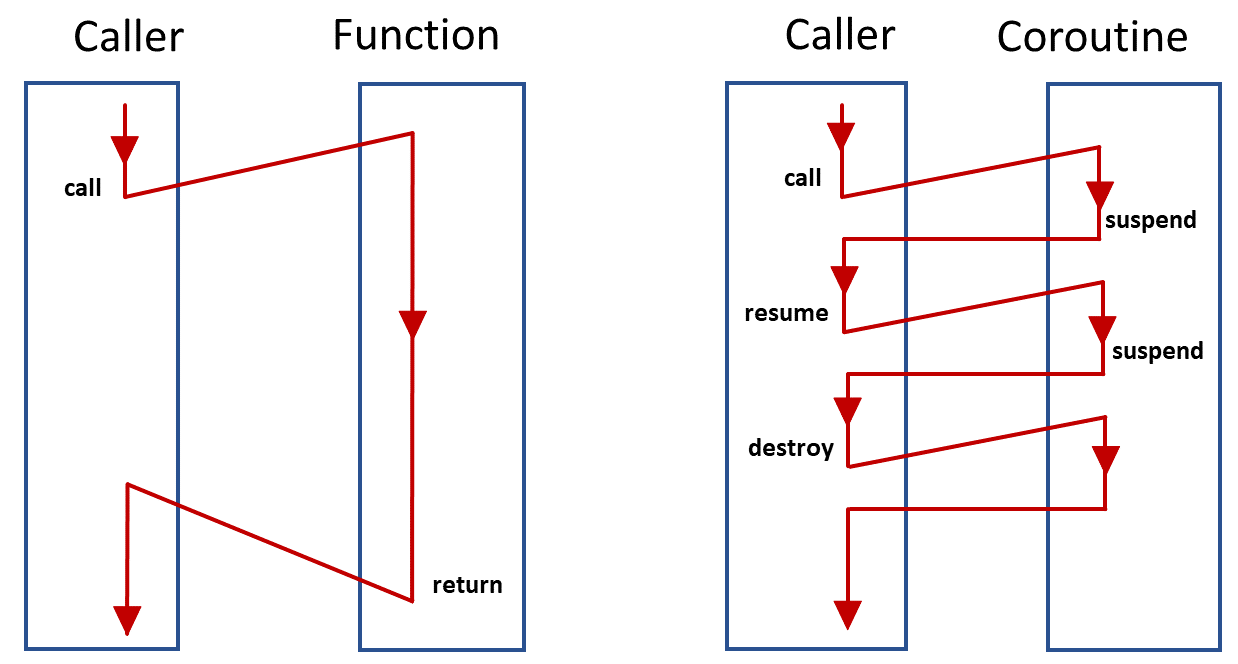
\includegraphics[width=0.8\textwidth]{content/3/chapter6/images/3.png}\\
函数与协程
\end{center}

(单线程中)调用函数只能等待其返回,但自使用协程时,可以将其挂起,之后再恢复它,并且可以销毁一个处于挂起状态的协程。

C++20使用新的关键字co\_await和co\_yield, 扩展了C++函数的执行方式。

co\_await表达式,可能暂停和恢复表达式的执行。使用co\_await表达式时,若函数的结果不可用,调用auto getResult = func()时不会阻塞。这里的阻塞,不是消耗资源的忙等,而是资源友好的等待。

co\_yield表达式支持生成器函数。每次调用生成器函数时,都会返回一个新值。生成器函数是一种数据流,可以从中选择值,数据流可以是无限的,这就是C++惰性求值的基础。

\subsubsubsection{6.1.1\hspace{0.2cm}生成器函数}

下面的程序非常简单。函数getNumbers会对范围内的整数加上对应的inc,并放在vector中返回。begin值必须小于end值,inc值必须为正。

\begin{lstlisting}[style=styleCXX]
// greedyGenerator.cpp

#include <iostream>
#include <vector>

std::vector<int> getNumbers(int begin, int end, int inc = 1) {

	std::vector<int> numbers;
	for (int i = begin; i < end; i += inc) {
		numbers.push_back(i);
	}
	
	return numbers;

}

int main() {

	std::cout << '\n';
	
	const auto numbers= getNumbers(-10, 11);
	
	for (auto n: numbers) std::cout << n << " ";
	
	std::cout << "\n\n";
	
	for (auto n: getNumbers(0, 101, 5)) std::cout << n << " ";
	
	std::cout << "\n\n";

}
\end{lstlisting}

这里,我用getNumbers重新发明了轮子,这项工作也可以用\href{http://en.cppreference.com/w/cpp/algorithm/iota}{std::iota}完成。

下面是输出。

\begin{center}
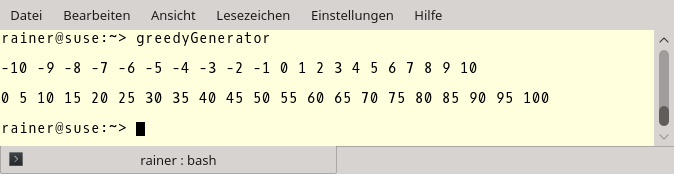
\includegraphics[width=0.8\textwidth]{content/3/chapter6/images/4.png}\\
\end{center}

我对greedyGenerator.cpp有两个观察。一是,第8行中的vector总会得到所有值。即使只对一个有1000个元素容器的前5个元素感兴趣,这也是成立的。二是,将函数getNumbers转换为惰性生成器很容易。以下程序是有意不完整显示的,这里生成器的定义仍然处于缺失状态。

\hspace*{\fill} \\ %插入空行
\noindent
\textbf{惰性生成器函数}
\begin{lstlisting}[style=styleCXX]
// lazyGenerator.cpp

#include <iostream>

generator<int> generatorForNumbers(int begin, int inc = 1) {

	for (int i = begin;; i += inc) {
		co_yield i;
	}

}

int main() {

	std::cout << '\n';
	
	const auto numbers = generatorForNumbers(-10);
	
	for (int i= 1; i <= 20; ++i) std::cout << numbers() << " ";
	
	std::cout << "\n\n";
	
	for (auto n: generatorForNumbers(0, 5)) std::cout << n << " ";
	
	std::cout << "\n\n";

}
\end{lstlisting}

getNumbers函数返回一个std::vector<int>(greedyGenerator.cpp),而协程generatorForNumbers会返回一个生成器(lazyGenerator.cpp)。第17行中的生成器数字或第23行中的generatorForNumbers(0,5)在请求时返回一个新数字。基于范围的for循环触发查询,协程的查询通过co\_yield i返回值i,并立即暂停其执行。若请求了一个新值,协程将在该位置恢复执行。

第23行中的表达式generatorForNumbers(0,5)是生成器的立即使用方式。我想明确强调,因为第8行中的for循环没有结束条件,所以协程生成器fornumbers可以创建无限的数据流。若只要求有限数量的值,但这对于第23行并不适用,因为没有结束条件,所以表达式会持续运行。

\subsubsubsection{6.1.2\hspace{0.2cm}特征}

协程有一些独有的特征。

\hspace*{\fill} \\ %插入空行
\noindent
\textbf{6.1.2.1\hspace{0.2cm}典型用例}

协程是编写\href{https://en.wikipedia.org/wiki/Event-driven_programming}{事件驱动应用}的常用方法,可以是模拟、游戏、服务器、用户界面,甚至算法。协程通常也用于\href{https://en.wikipedia.org/wiki/Computer_multitasking}{协作多任务处理}。协作多任务处理的关键是,每个任务都需要尽可能多的时间,不休眠或等待,而是允许其他任务运行。合作多任务与抢占式多任务相反,抢占式多任务有一个调度程序,需要决定每个任务占用CPU的时间。

当然,也有各种类型的协程。

\hspace*{\fill} \\ %插入空行
\noindent
\textbf{6.1.2.2\hspace{0.2cm}基本概念}

C++20中的协程是不对称的、头等的、无堆栈的。

非对称协程的工作流程会直接返回至调用方,这并不适用于对称协程。对称协程可以将其工作流委托给另一个协程。

头等协程类似于头等函数,因为协程的行为类似于数据,所以可以将它们用作函数的参数或从函数返回值,或将它们存储在变量中。

无堆栈协程可以挂起和恢复顶层协程。协程的执行和协程的产物返回给调用方,协程将其恢复状态与堆栈分开存储。无堆栈协程通常称为可恢复函数。

\hspace*{\fill} \\ %插入空行
\noindent
\textbf{6.1.2.3\hspace{0.2cm}设计目的}

Gor Nishanov在提案\href{https://isocpp.org/files/papers/N4402.pdf}{N4402}中描述了协程的设计目的。

协程应该是

\begin{itemize}
\item 
高度可扩展(可并发数十亿个协程)

\item 
具有高效的恢复和暂停操作,并且成本与功能的开销相当

\item 
与现有设施无缝交互,没有开销

\item 
开放的协程机制允许库设计者开发协程库,公开各种高级语义,如生成器、\href{https://tour.golang.org/concurrency/1}{goroutines}、任务等

\item 
可用于禁止异常不可用的环境
\end{itemize}

因为可扩展性和与现有设施的无缝交互的设计目标,所以协程是无堆栈的。相反,堆栈协程在Windows上会有1MB大小的默认堆栈,在Linux上有2MB大小的默认堆栈。

一个函数有四种方式可以成为协程。

\hspace*{\fill} \\ %插入空行
\noindent
\textbf{6.1.2.4\hspace{0.2cm}成为协程}

若函数使用了协程,就成为了协程

\begin{itemize}
\item 
co\_return, 或

\item 
co\_await, 或

\item 
co\_yield, 或

\item 
基于范围的for循环中的co\_await表达式。
\end{itemize}

\begin{tcolorbox}[breakable,enhanced jigsaw,colback=red!5!white,colframe=red!75!black,title={协程工厂和协程对象的区别}]
	
协程这个术语通常用于两个不同方面:调用co\_return、co\_await或co\_yield的函数,以及协程对象。用一个术语表示两个不同的协程方面,可能会让读者感到困惑(就像我一样)。先来说一下这两个术语。

\hspace*{\fill} \\ %插入空行
\noindent
\textbf{生成2021的协程}
\begin{lstlisting}[style=styleCXX]
MyFuture<int> createFuture() {
	co_return 2021;
}

int main() {
	
	auto fut = createFuture();
	std::cout << "fut.get(): " << fut.get() << '\n';
	
}
\end{lstlisting}

例子中有一个createFuture函数,返回一个MyFuture<int>类型的对象,两者都称为协程。createFuture函数是一个返回协程对象的协程工厂。协程对象是一个可恢复的对象,是对特定行为建模的框架。我在co\_return一节中会介绍这个简单的协程的实现和使用。
	
\end{tcolorbox}

\hspace*{\fill} \\ %插入空行
\noindent
\textbf{6.1.2.4.1 \hspace{0.2cm}限制}

协程不能有返回语句或占位符返回类型,这适用于无约束占位符(auto)和有约束占位符(concepts)。

此外,具有\href{https://en.cppreference.com/w/cpp/language/variadic_arguments}{可变参数}、constexpr函数、consteval函数、构造函数、析构函数和main函数的函数不能是协程。

\subsubsubsection{6.1.3\hspace{0.2cm}架构}

实现协程的框架由20多个函数组成,其中一些必须实现,一些可以重载。因此,可以根据需要定制协程。

协程有三个重要部分:promise对象、协程句柄和协程帧。用户获得的协程句柄,可以与promise对象交互,promise对象将其状态保存在协程帧中。

\begin{center}
Promise对象
\end{center}

\begin{table}[H]
\centering
\begin{tabular}{ll}
\textbf{成员函数}  & \textbf{描述}                                 \\ \hline
默认构造函数       & Promise必须是默认可构造的。             \\
initial\_suspend()        & 确定协程在运行前是否挂起。 \\
final\_suspend noexcept() & 确定协程在结束前是否挂起。 \\
unhandled\_exception()    & 发生异常时使用。                    \\
get\_return\_object()     & 返回协程对象(可恢复对象)。     \\
return\_value(val)        & 等价于co\_return val。                        \\
return\_void()            & 等价于co\_return。                            \\
yield\_value(val)         & 等价于co\_yield val。                        
\end{tabular}
\end{table}

编译器在执行协程期间会自动调用这些函数。

get\_return\_object返回调用端,用来与协程交互的可恢复对象。promise至少需要一个成员函数return\_value、return\_void或yield\_value。若协程永不结束,则不需要定义成员函数return\_value或return\_void。

这三个函数yield\_value、initial\_suspend和final\_suspend返回可等待对象。可等待对象表示需要对其行为进行等待的对象,且可等待属性决定协程是否可以暂停。

\hspace*{\fill} \\ %插入空行
\noindent
\textbf{6.1.3.2\hspace{0.2cm}协程句柄}

协程句柄是一个非自有句柄,用于从外部恢复或销毁协程帧。协程句柄是可恢复函数的一部分。

下面的代码段展示了一个具有协程句柄coro的简单Generator对象。

\begin{lstlisting}[style=styleCXX]
template<typename T>
struct Generator {

	struct promise_type;
	using handle_type = std::coroutine_handle<promise_type>;
	
	Generator(handle_type h): coro(h) {}
	handle_type coro;
	
	~Generator() {
		if ( coro ) coro.destroy();
	}
	T getValue() {
		return coro.promise().current_value;
	}
	bool next() {
		coro.resume();
		return not coro.done();
	}
	...
}
\end{lstlisting}

构造函数(第7行)获取类型为\href{https://en.cppreference.com/w/cpp/coroutine/coroutine_handle}{std::coroutine\_handle<promise\_type>}的promise的协程句柄。成员函数next(第16行)和getValue(第13行)允许调用端使用协程句柄恢复promise(gen.next())或获取其值(gen.getValue())。

\hspace*{\fill} \\ %插入空行
\noindent
\textbf{调用协程}
\begin{lstlisting}[style=styleCXX]
Generator<int> coroutineFactory(); // function that returns a coroutine object

auto gen = coroutineFactory();
gen.next();
auto result = gen.getValue();
\end{lstlisting}

在内部,两个函数都会使用协程句柄coro(第8行)

\begin{itemize}
\item 
恢复协程:coro.resume()(第17行)或coro();

\item 
销毁协程:coro.destroy()(第11行);

\item 
检查协程的状态:coro(第11行)。
\end{itemize}

协程在其函数体结束时自动销毁,调用coro会在其最终挂起点返回true。

\begin{tcolorbox}[breakable,enhanced jigsaw,colback=red!5!white,colframe=red!75!black,title={可恢复对象需要内部类型promise\_type}]
可恢复对象(例如:Generator)必须有一个内部类型promise\_type。或者,可以特化Generator上的\href{https://en.cppreference.com/w/cpp/coroutine/coroutine_traits}{std::coroutine\_traits},并在其中定义一个公共成员promise\_type: std::coroutine\_traits<Generator>。
\end{tcolorbox}

\hspace*{\fill} \\ %插入空行
\noindent
\textbf{6.1.3.3\hspace{0.2cm}协程帧}

协程帧在内部使用,通常由堆分配。它由前面提到的promise对象、协程复制的参数、挂起点、当前挂起点之前生命周期结束的局部变量,以及生命周期超过当前挂起点的局部变量组成。

优化协程的分配有两个必要条件:

\begin{enumerate}
\item 
协程的生存期必须嵌套在调用者的生存期内

\item 
协程的调用者知道协程帧的大小。

\end{enumerate}

\subsubsubsection{6.1.4\hspace{0.2cm}可等待类型和具有等待模式的类型}

promise对象的三个函数分别yield\_value、initial\_suspend和final\_suspend返回可等待对象。

\hspace*{\fill} \\ %插入空行
\noindent
\textbf{6.1.4.1\hspace{0.2cm}可等待类型}

可等待对象表示需要对其行为进行等待的对象。并且,可等待属性决定协程是否可以暂停。

实际上,编译器使用promise prom和co\_await操作符生成了三个函数调用。

\begin{center}
编译器生成的函数调用
\end{center}

\begin{table}[H]
\centering
\begin{tabular}{ll}
\textbf{函数调用}           & \textbf{编译器生成的调用}   \\ \hline
yield value             & co\_await prom.yield\_value(value) \\
prom.initial\_suspend() & co\_await prom.initial\_suspend()  \\
prom.final\_suspend()   & co\_await prom.final\_suspend()   
\end{tabular}
\end{table}

co\_await操作符需要一个可等待对象as参数。

\hspace*{\fill} \\ %插入空行
\noindent
\textbf{6.1.4.2\hspace{0.2cm}可等待的概念}

可等待的概念需要三个功能。

\begin{center}
可等待的概念
\end{center}

\begin{table}[H]
\centering
\begin{tabular}{ll}
\textbf{函数} & \textbf{描述}                                  \\ \hline
await\_ready & \begin{tabular}[c]{@{}l@{}}指示结果是否已准备好。当它返回false时,\\ 将调用await\_suspend。\end{tabular} \\ \hline
await\_suspend    & 将协程调度状态改为恢复或销毁。 \\ \hline
await\_resume     & 提供co\_await exp表达式的结果。\\ \hline
\end{tabular}
\end{table}

C++20标准定义了两个基本的可等待对象:std::suspend\_always和std::suspend\_never。

\hspace*{\fill} \\ %插入空行
\noindent
\textbf{6.1.4.3\hspace{0.2cm}std::suspend\_always和std::suspend\_never}

顾名思义,std::suspend\_always总是挂起,调用await\_ready会返回false。

\begin{lstlisting}[style=styleCXX]
struct suspend_always {
	constexpr bool await_ready() const noexcept { return false; }
	constexpr void await_suspend(std::coroutine_handle<>) const noexcept {}
	constexpr void await_resume() const noexcept {}
};
\end{lstlisting}

相反的情况是std::suspend\_never,调用await\_ready会返回true。

\begin{lstlisting}[style=styleCXX]
struct suspend_never {
	constexpr bool await_ready() const noexcept { return true; }
	constexpr void await_suspend(std::coroutine_handle<>) const noexcept {}
	constexpr void await_resume() const noexcept {}
};
\end{lstlisting}

可等待对象std::suspend\_always和std::suspend\_never是函数的基本构建块,例如:initial\_suspend和final\_suspend。这两个函数在协程执行时自动执行:initial\_suspend在协程的开始执行,final\_suspend在协程的结束执行。

\hspace*{\fill} \\ %插入空行
\noindent
\textbf{6.1.4.4\hspace{0.2cm}initial\_suspend}

成员函数initial\_suspend返回std::suspend\_always时,协程将从其开始处挂起。当返回std::suspend\_never时,协程不会暂停。

\begin{itemize}
\item 
立即暂停的惰性协程

\begin{lstlisting}[style=styleCXX]
std::suspend_always initial_suspend() {
	return {};
}
\end{lstlisting}

\item 
立即运行的立即协程

\begin{lstlisting}[style=styleCXX]
std::suspend_never initial_suspend() {
	return {};
}
\end{lstlisting}
\end{itemize}


\hspace*{\fill} \\ %插入空行
\noindent
\textbf{6.1.4.5\hspace{0.2cm}final\_suspend}

成员函数final\_suspend返回std::suspend\_always时,协程将在结束时挂起。当返回std::suspend\_never时,协程不会暂停。

\begin{itemize}
\item 
结束时暂停的惰性协程

\begin{lstlisting}[style=styleCXX]
std::suspend_always final_suspend() noexcept {
	return {};
}
\end{lstlisting}

\item 
立即协程不会在结束时暂停

\begin{lstlisting}[style=styleCXX]
std::suspend_never final_suspend() noexcept {
	return {};
}
\end{lstlisting}
\end{itemize}

现在,我们只有可等待对象,但我们需要一些东西来进行等待。让我来填补空缺,就是写一篇关于Awaiters的文章。

\hspace*{\fill} \\ %插入空行
\noindent
\textbf{6.1.4.6\hspace{0.2cm}待等待类型(Awaiter,具有等待模式的类型)}

有两种方法获取待等待对象。

\begin{itemize}
\item 
定义co\_await操作符。

\item 
将可等待对象变为待等待对象。
\end{itemize}

当使用co\_await表达式时,该表达式是一个可等待表达式。此外,表达式是对promise对象(可等待)的调用:prom.yield\_value(value)、prom.initial\_suspend()或prom.final\_suspend()。为了可读性,我在以下几行中将promise对象prom重命名为awaitable。

现在,编译器执行以下查找规则来获取待等待对象:

\begin{enumerate}
\item 
在promise对象上查找co\_await操作符,并返回一个awaiter:
\begin{lstlisting}[style=styleCXX]
awaiter = awaitable.operator co_await();
\end{lstlisting}

\item 
寻找一个独立的co\_wait操作符,并返回一个awaiter:
\begin{lstlisting}[style=styleCXX]
awaiter = operator co_await();
\end{lstlisting}

\item 
若没有定义co\_wait操作符,awaitable就成为awaiter:
\begin{lstlisting}[style=styleCXX]
awaiter = awaitable;
\end{lstlisting}
\end{enumerate}

\begin{tcolorbox}[breakable,enhanced jigsaw,colback=blue!5!white,colframe=blue!75!black,title={awaiter = awaitable}]
本章学习协程实现时,可能会注意大部分示例都将使awaitable隐式地变成awaiter。只有线程同步的例子使用了co\_await操作符来获取待等待对象。
\end{tcolorbox}

了解了协程的静态特性后,继续来看看其动态特性。

\subsubsubsection{6.1.5\hspace{0.2cm}工作流}

编译器转换协程,并运行两个工作流:外部promise工作流和内部awaiter工作流。

\hspace*{\fill} \\ %插入空行
\noindent
\textbf{6.1.5.1\hspace{0.2cm}Promise工作流}

在一个函数中使用co\_yield、co\_await或co\_return时,这个函数就变成了协程,编译器就会把其主体转换成类似于下面这行代码的东西。

\hspace*{\fill} \\ %插入空行
\noindent
\textbf{转换后的协程}
\begin{lstlisting}[style=styleCXX]
{
	Promise prom;
	co_await prom.initial_suspend();
	try {
		<function body having co_return, co_yield, or co_wait>
	}
	catch (...) {
		prom.unhandled_exception();
	}
FinalSuspend:
	co_await prom.final_suspend();
}
\end{lstlisting}

编译器使用promise对象的函数自动运行转换后的代码,我把这个工作流称为promise工作流。下面是这个工作流的主要步骤:

\begin{itemize}
\item 
协程开始执行

\begin{itemize}
\item 
若需要,可以分配协程帧

\item 
将所有函数参数复制到协程帧

\item 
创建prom(第2行)

\item 
调用prom.get\_return\_object()创建协程句柄,将其保存在局部变量中。协程第一次挂起时,调用的结果将返回给调用方。

\item 
调用prom.initial\_suspend(),并co\_await其结果。promise类型通常对急于启动的协程返回suspend\_never,对惰性启动的协程则返回suspend\_always。(第3行)

\item 
协程的主体在co\_await prom.initial\_suspend()恢复时执行
\end{itemize}

\item 
协程到达一个暂停点
\begin{itemize}
\item 
返回对象(prom.get\_return\_object())返回给恢复协程的调用者
\end{itemize}

\item 
协程达到co\_return
\begin{itemize}
\item 
为co\_return或co\_return表达式调用prom.return\_void(),其中表达式类型为void

\item 
为co\_return表达式调用prom.return\_value(expression),其中表达式具有非void类型。

\item 
销毁所有在堆栈上创建的变量

\item 
调用prom.final\_suspend(),并co\_await其结果
\end{itemize}

\item 
销毁协程(通过co\_return一个未捕获的异常终止,或者通过协程句柄终止)
\begin{itemize}
\item 
调用promise对象的销毁

\item 
调用函数参数的析构函数

\item 
释放协程帧使用的内存

\item 
将控制权转回调用方
\end{itemize}
\end{itemize}

当协程以未捕获的异常结束时,会发生以下情况:

\begin{itemize}
\item 
捕获异常并从捕获块调用prom.unhandled\_exception()

\item 
调用prom.final\_suspend()和co\_await(第11行)
\end{itemize}

在协程中使用co\_await expr时,或者编译器隐式调用co\_await prom.initial\_suspend()、co\_await prom.final.suspend()或co\_await prom.yield\_value(value)时,第二个内部awaiter工作流将启动。

\hspace*{\fill} \\ %插入空行
\noindent
\textbf{6.1.5.2\hspace{0.2cm}awaiter工作流}

使用co\_await expr会使编译器基于await\_ready、await\_suspend和await\_resume函数来转换代码,所以我将转换后的代码的执行称为awaiter工作流。

编译器使用可等待方式生成大致如下的代码,我忽略了异常处理,并使用注释描述了工作流。

\hspace*{\fill} \\ %插入空行
\noindent
\textbf{生成的awaiter工作流}
\begin{lstlisting}[style=styleCXX]
awaitable.await_ready() returns false:

	suspend coroutine
	
	awaitable.await_suspend(coroutineHandle) returns:
		void:
			awaitable.await_suspend(coroutineHandle);
			coroutine keeps suspended
			return to caller
	
		bool:
			bool result = awaitable.await_suspend(coroutineHandle);
			if result:
				coroutine keep suspended
				return to caller
			else:
				go to resumptionPoint
	
		another coroutine handle:
			auto anotherCoroutineHandle = awaitable.await_suspend(coroutineHandle);
			anotherCoroutineHandle.resume();
			return to caller

resumptionPoint:

return awaitable.await_resume();
\end{lstlisting}

只有当awaitable.await\_ready()返回false(第1行)时,工作流才会执行。若返回true,协程已经准备就绪,并返回调用awaitable.await\_resume()的结果(第26行)。

假设awaitable.await\_ready()返回false。首先,将协程挂起(第3行),并立即计算awaitable.await\_suspend()的返回值。返回类型可以是void(第6行)、布尔值(第11行)或另一个协程句柄(第19行),例如:anotherCoroutineHandle。根据返回类型,程序流返回或执行另一个协程。

\begin{center}
返回awaitable.await\_suspend()的值
\end{center}

\begin{table}[H]
\centering
\begin{tabular}{ll}
\textbf{类型}          & \textbf{描述}                                      \\ \hline
void                   & 协程保持挂起,并将运行权返回给调用者。  \\ \hline
bool &
\begin{tabular}[c]{@{}l@{}}bool == true:协程保持挂起,并将运行权返回给调用者。\\ bool == false:协程恢复,运行权不返回给调用方。\end{tabular} \\ \hline
anotherCoroutineHandle & 恢复另一个协程,并将运行权返回给调用方。 \\ \hline
\end{tabular}
\end{table}

若抛出异常会发生什么?若异常发生在await\_ready、await\_suspend或await\_resume中,情况会有所不同。

\begin{itemize}
\item 
await\_ready: 协程不会挂起,也不会计算await\_suspend或await\_resume。

\item 
await\_suspend: 异常捕获,协程恢复,异常重新抛出。不调用await\_resume。

\item 
await\_resume: await\_ready和await\_suspend计算并返回所有值。当然,await\_resume的调用并不返回结果。
\end{itemize}

好了,来把理论付诸至实践吧。

\subsubsubsection{6.1.6\hspace{0.2cm}co\_return}

协程使用co\_return作为返回语句。

\hspace*{\fill} \\ %插入空行
\noindent
\textbf{6.1.6.1\hspace{0.2cm}future}

不可否认,下面的eagerFuture.cpp中的协程是我能想象到的最简单的协程。就算这样,它还是可以做一些有意义的事情:自动存储调用结果。

\begin{lstlisting}[style=styleCXX]
// eagerFuture.cpp

#include <coroutine>
#include <iostream>
#include <memory>

template<typename T>
struct MyFuture {
	std::shared_ptr<T> value;
	MyFuture(std::shared_ptr<T> p): value(p) {}
	~MyFuture() { }
		T get() {
		return *value;
	}

	struct promise_type {
		std::shared_ptr<T> ptr = std::make_shared<T>();
		~promise_type() { }
		MyFuture<T> get_return_object() {
			return ptr;
		}
		void return_value(T v) {
			*ptr = v;
		}
		std::suspend_never initial_suspend() {
			return {};
		}
		std::suspend_never final_suspend() noexcept {
			return {};
		}
		void unhandled_exception() {
			std::exit(1);
		}
	};
};

MyFuture<int> createFuture() {
	co_return 2021;
}

int main() {

	std::cout << '\n';
	
	auto fut = createFuture();
	std::cout << "fut.get(): " << fut.get() << '\n';
	
	std::cout << '\n';

}
\end{lstlisting}

MyFuture的行为和\href{https://en.cppreference.com/w/cpp/thread/future}{future}很像,会立即运行。调用协程createFuture(第45行)返回future,调用fut.get(第46行)获取相关promise中的结果。

与future有一个微妙的区别,协程createFuture的返回值在调用后可用。由于生命周期问题,返回值由std::shared\_ptr管理(第9行和第17行)。协程总是使用std::suspend\_never(第25行和第28行),因为在运行前后都不会挂起,所以在调用createFuture函数时可以执行协程。成员函数get\_return\_object(第19行)创建并存储协程对象的句柄,return\_value(第22行)存储协程的结果,该结果由co\_return 2021(第38行)提供。调用端使用fut.get(第46行),并使用future作为promise的句柄。成员函数get将结果返回给调用端(第13行)。

\begin{tcblisting}{commandshell={}}
fut.get(): 2021
\end{tcblisting}

有读者可能认为,不值得花费精力实现一个行为就像函数一样的协程。你说得没错!然而,这个简单的协程是编写各种future实现的起点。第7章中,可以看到更多future的变体。

\subsubsubsection{6.1.7\hspace{0.2cm}co\_yield}

使用co\_yield,可以实现一个生成器,生成无限数据流,可以连续查询值。生成器generatorForNumbers(int begin, int inc= 1)的返回类型是generator<int>,其中generator内部持有一个特殊的promise p,使得使用co\_yield i等价于使用co\_await p.yield\_value(i)。语句co\_yield i可以使用任意次。每次使用后,协程会立即挂起。

\hspace*{\fill} \\ %插入空行
\noindent
\textbf{6.1.7.1\hspace{0.2cm}无限的数据流}

infiniteDataStream.cpp产生一个无限数据流。协程getNext使用co\_yield创建一个数据流,该数据流从start开始,并在请求时给出按步递增的下一个值。

\begin{lstlisting}[style=styleCXX]
// infiniteDataStream.cpp

#include <coroutine>
#include <memory>
#include <iostream>

template<typename T>
struct Generator {

	struct promise_type;
	using handle_type = std::coroutine_handle<promise_type>;
	
	Generator(handle_type h): coro(h) {} // (3)
	handle_type coro;
	
	~Generator() {
		if ( coro ) coro.destroy();
	}

	Generator(const Generator&) = delete;
	Generator& operator = (const Generator&) = delete;
	Generator(Generator&& oth) noexcept : coro(oth.coro) {
		oth.coro = nullptr;
	}
		Generator& operator = (Generator&& oth) noexcept {
		coro = oth.coro;
		oth.coro = nullptr;
		return *this;
	}
	T getValue() {
		return coro.promise().current_value;
	}
	bool next() { // (5)
		coro.resume();
		return not coro.done();
	}
	struct promise_type {
		promise_type() = default; // (1)
		
		~promise_type() = default;
		
		auto initial_suspend() { // (4)
			return std::suspend_always{};
		}
		auto final_suspend() noexcept {
			return std::suspend_always{};
		}
		auto get_return_object() { // (2)
			return Generator{handle_type::from_promise(*this)};
		}
		auto return_void() {
			return std::suspend_never{};
		}
	
		auto yield_value(const T value) { // (6)
			current_value = value;
			return std::suspend_always{};
		}
		void unhandled_exception() {
			std::exit(1);
		}
		T current_value;
	};

};

Generator<int> getNext(int start = 0, int step = 1) {
	auto value = start;
	while (true) {
		co_yield value;
		value += step;
	}
}

int main() {

	std::cout << '\n';
	
	std::cout << "getNext():";
	auto gen = getNext();
	for (int i = 0; i <= 10; ++i) {
		gen.next();
		std::cout << " " << gen.getValue(); // (7)
	}
	
	std::cout << "\n\n";
	
	std::cout << "getNext(100, -10):";
	auto gen2 = getNext(100, -10);
	for (int i = 0; i <= 20; ++i) {
		gen2.next();
		std::cout << " " << gen2.getValue();
	}
	
	std::cout << '\n';

}
\end{lstlisting}

主程序创建了两个协程。第一个gen(第80行)返回从0到10的值,第二个gen2(第89行)返回从100到-100的值。在深入了解工作流程之前,可以在在线编译器\href{https://wandbox.org/}{Wandbox}上尝试这段程序,下面是程序的输出。

\begin{center}
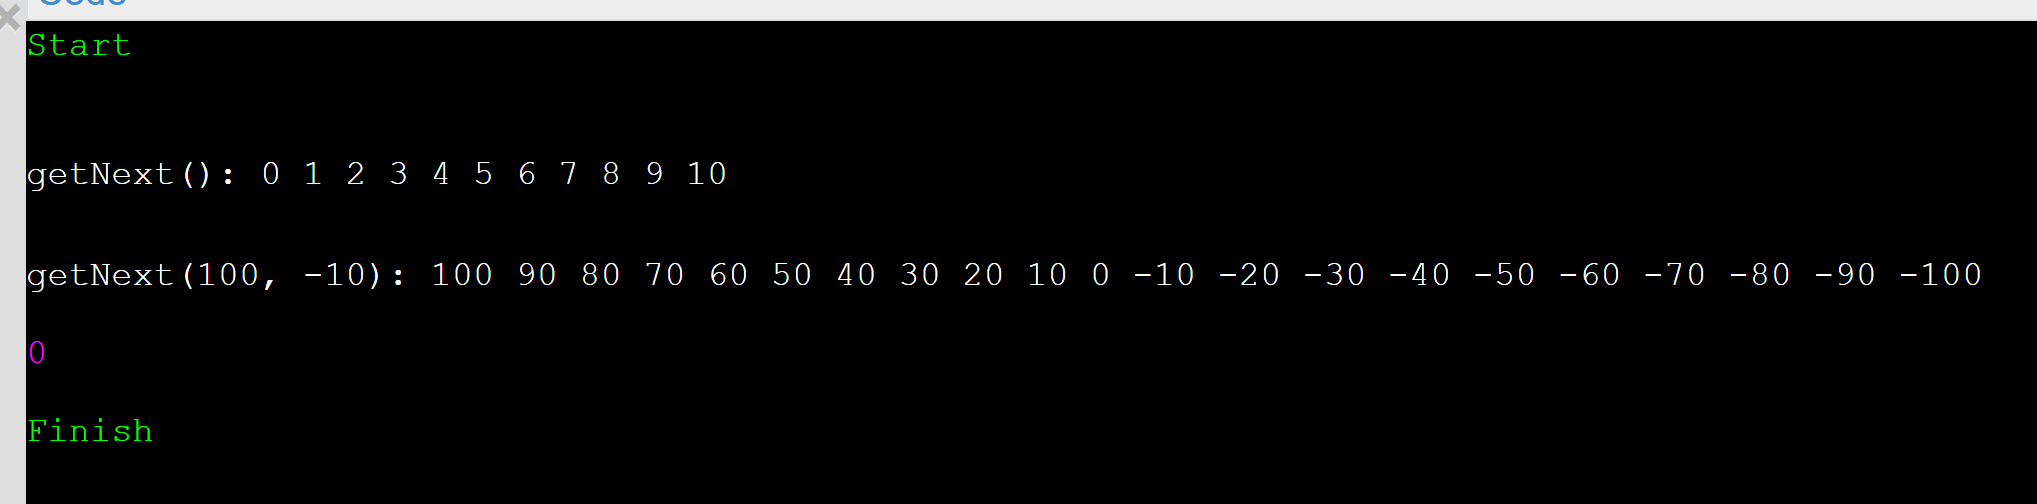
\includegraphics[width=0.8\textwidth]{content/3/chapter6/images/5.png}\\
\end{center}

infinitedatstream.cpp中的数字代表工作流第一次迭代中的步骤。

\begin{enumerate}
\item 
创建promise

\item 
调用promise.get\_return\_object(),并将结果保存在一个局部变量中

\item 
创建生成器

\item 
调用promise.initial\_suspend()。生成器是惰性的,因此总是挂起。

\item 
请求下一个值,若生成器已用完,则直接返回。

\item 
由co\_yield触发调用,下一个值在此之后可用。

\item 
获取下一个值
\end{enumerate}

其他迭代中,只执行步骤5、6和7。

第7章中的线程的修改和泛化讨论了生成器infinitdataststream.cpp的进一步改进和修改

\subsubsubsection{6.1.8\hspace{0.2cm}co\_await}

co\_await会使协程的执行暂停或恢复。co\_await exp中的表达式exp必须是可等待的表达式,即必须实现一个特定的接口,由await\_ready、await\_suspend和await\_resume三个函数组成。

co\_await的典型用例是等待事件的服务器。

\hspace*{\fill} \\ %插入空行
\noindent
\textbf{阻塞式服务器}
\begin{lstlisting}[style=styleCXX]
Acceptor acceptor{443};
while (true) {
	Socket socket = acceptor.accept(); // blocking
	auto request = socket.read(); // blocking
	auto response = handleRequest(request);
	socket.write(response); // blocking
}
\end{lstlisting}

服务器非常简单,因为在同一个线程中依次回答每个请求。服务器监听443端口(第1行),接受连接(第3行),从客户端读取传入数据(第4行),并将其答案写入客户端(第6行)。第3、4和6行的调用是阻塞的。

因为co\_await,所以阻塞调用现在可以挂起并恢复。

\hspace*{\fill} \\ %插入空行
\noindent
\textbf{等待式服务器}
\begin{lstlisting}[style=styleCXX]
Acceptor acceptor{443};
while (true) {
	Socket socket = co_await acceptor.accept();
	auto request = co_await socket.read();
	auto response = handleRequest(request);
	co_await socket.write(response);
}
\end{lstlisting}

介绍使用协程进行线程同步的示例之前,我想先从一些简单的事情开始:根据请求进行启动。

\hspace*{\fill} \\ %插入空行
\noindent
\textbf{6.1.8.1\hspace{0.2cm}根据请求进行启动}

下面示例中的协程非常简单,等待预定义的std::suspend\_never()。

\hspace*{\fill} \\ %插入空行
\noindent
\textbf{根据请求进行启动}
\begin{lstlisting}[style=styleCXX]
// startJob.cpp

#include <coroutine>
#include <iostream>

struct Job {
	struct promise_type;
	using handle_type = std::coroutine_handle<promise_type>;
	handle_type coro;
	Job(handle_type h): coro(h){}
	~Job() {
		if ( coro ) coro.destroy();
	}
	void start() {
		coro.resume();
	}


	struct promise_type {
		auto get_return_object() {
			return Job{handle_type::from_promise(*this)};
		}
		std::suspend_always initial_suspend() {
			std::cout << " Preparing job" << '\n';
			return {};
		}
		std::suspend_always final_suspend() noexcept {
			std::cout << " Performing job" << '\n';
			return {};
		}
		void return_void() {}
		void unhandled_exception() {}
	
	};
};

Job prepareJob() {
	co_await std::suspend_never();
}

int main() {

	std::cout << "Before job" << '\n';
	
	auto job = prepareJob();
	job.start();
	
	std::cout << "After job" << '\n';

}
\end{lstlisting}

有读者可能认为协程prepareJob(第37行)没有意义,因为可等待对象总是挂起。不!函数prepareJob至少是一个使用co\_await(第38行),并返回一个协程对象的协程工厂。第45行中的函数调用prepareJob()创建了Job类型的协程对象。了解数据类型Job时,会发现协程对象立即挂起,因为promise的成员函数返回std::suspend\_always(第23行),这正是函数启动作业的原因。start(第46行)是恢复协程(第15行)所必需的,成员函数final\_suspend也返回std::suspend\_always(第27行)。

\begin{tcblisting}{commandshell={}}
Before job
    Preparing job
    Performing job
After job
\end{tcblisting}

第7章的作业流部分,我将使用startJob程序作为进一步实验的案例。

\hspace*{\fill} \\ %插入空行
\noindent
\textbf{6.1.8.2\hspace{0.2cm}线程同步}

这是典型的线程同步,一个线程准备另一个线程等待的工作包。\href{https://en.cppreference.com/w/cpp/thread/condition_variable}{条件变量}, \href{https://en.cppreference.com/w/cpp/thread}{promises和future},以及\href{https://en.cppreference.com/w/cpp/atomic/atomic}{原子布尔类型}都可以用来创建发送方-接收方工作流。因为协程可用,所以线程同步变得非常容易,避免了条件变量的风险,比如:伪唤醒和未唤醒。

\begin{lstlisting}[style=styleCXX]
// senderReceiver.cpp

#include <coroutine>
#include <chrono>
#include <iostream>
#include <functional>
#include <string>
#include <stdexcept>
#include <atomic>
#include <thread>

class Event {
public:
	Event() = default;

	Event(const Event&) = delete;
	Event(Event&&) = delete;
	Event& operator=(const Event&) = delete;
	Event& operator=(Event&&) = delete;

	class Awaiter;
	Awaiter operator co_await() const noexcept;
	
	void notify() noexcept;

private:

	friend class Awaiter;
	
	mutable std::atomic<void*> suspendedWaiter{nullptr};
	mutable std::atomic<bool> notified{false};

};

class Event::Awaiter {
public:
	Awaiter(const Event& eve): event(eve) {}
	
	bool await_ready() const;
	bool await_suspend(std::coroutine_handle<> corHandle) noexcept;
	void await_resume() noexcept {}

private:
	friend class Event;
	
	const Event& event;
	std::coroutine_handle<> coroutineHandle;
};

bool Event::Awaiter::await_ready() const {

	// allow at most one waiter
	if (event.suspendedWaiter.load() != nullptr){
		throw std::runtime_error("More than one waiter is not valid");
	}
	
	// event.notified == false; suspends the coroutine
	// event.notified == true; the coroutine is executed like a normal function
	return event.notified;
}

bool Event::Awaiter::await_suspend(std::coroutine_handle<> corHandle) noexcept {

	coroutineHandle = corHandle;
	
	if (event.notified) return false;
	
	// store the waiter for later notification
	event.suspendedWaiter.store(this);
	
	return true;
}

void Event::notify() noexcept {
	notified = true;
	
	// try to load the waiter
	auto* waiter = static_cast<Awaiter*>(suspendedWaiter.load());
	
	// check if a waiter is available
	if (waiter != nullptr) {
		// resume the coroutine => await_resume
		waiter->coroutineHandle.resume();
	}
}

Event::Awaiter Event::operator co_await() const noexcept {
	return Awaiter{ *this };
}

struct Task {
	struct promise_type {
		Task get_return_object() { return {}; }
		std::suspend_never initial_suspend() { return {}; }
		std::suspend_never final_suspend() noexcept { return {}; }
		void return_void() {}
		void unhandled_exception() {}
	};
};

Task receiver(Event& event) {
	auto start = std::chrono::high_resolution_clock::now();
	co_await event;
	std::cout << "Got the notification! " << '\n';
	auto end = std::chrono::high_resolution_clock::now();
	std::chrono::duration<double> elapsed = end - start;
	std::cout << "Waited " << elapsed.count() << " seconds." << '\n';
}

using namespace std::chrono_literals;

int main() {
	
	std::cout << '\n';
	
	std::cout << "Notification before waiting" << '\n';
	Event event1{};
	auto senderThread1 = std::thread([&event1]{ event1.notify(); }); // Notification
	auto receiverThread1 = std::thread(receiver, std::ref(event1));
	
	receiverThread1.join();
	senderThread1.join();
	
	std::cout << '\n';
	
	std::cout << "Notification after 2 seconds waiting" << '\n';
	Event event2{};
	auto receiverThread2 = std::thread(receiver, std::ref(event2));
	auto senderThread2 = std::thread([&event2]{
		std::this_thread::sleep_for(2s);
		event2.notify(); // Notification
	});
	
	receiverThread2.join();
	senderThread2.join();
	
	std::cout << '\n';
	
}
\end{lstlisting}

让我们看一下senderReceiver.cpp。线程senderThread1(第119行)和senderThread2(第130行)分别在第119行和第132行中使用一个事件发送通知。第102-109行中的函数receiver是协程,在线程receiverThread1(第122行)和receiverThread2(第135行)中执行。我统计了协程开始和结束之间的时间,并将其显示出来。这个数字显示了协程等待的时间,下面的屏幕截图显示了程序的输出。

\begin{center}
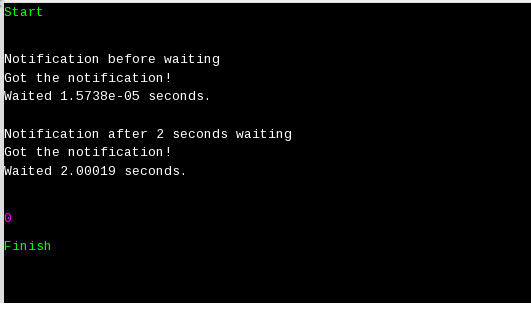
\includegraphics[width=0.6\textwidth]{content/3/chapter6/images/6.png}\\
线程同步
\end{center}

若将无限数据流中的类Generator与本例中的类Event进行比较,就会发现细微的差异。第一种情况下,生成器是可等待的和待等待的;第二种情况下,事件使用操作符co\_await返回待等待对象。这种将关注点分离为可等待对象和待等待对象的方法,改善了代码结构。

输出显示第二个协程的执行大约需要两秒钟。原因是event1在协程挂起之前发送了通知(第119行),而event2在2秒(第132行)后才发送的通知。

现在,切换为实现者角色。协程的工作流程确实很难掌控。类Event有两个有趣的成员:suspendedWaiter和notified。第31行中的变量suspendedWaiter保存了信号的等待器,第32行中的notify具有通知的状态。

在对这两个工作流的解释中,假设在第一种情况下(第一个工作流),事件通知发生在协程等待事件之前。对于第二种情况(第二个工作流),假设正好相反。

先来看看event1和第一个工作流,event1在启动receiverThread1之前发送通知。调用event1(第118行)触发notify(第75行)。设置通知标志,然后调用static\_cast<Awaiter*>(suspendedWaiter.load());装载waiter。本例中,waiter是nullptr,因为之前没有设置,所以不会执行第84行中对waiter的以下恢复调用。随后执行函数await\_ready(第51行)首先检查是否有多个waiter,若是的话抛出std::runtime异常,该方法的关键部分是返回值。event.notification已经在notify方法中设置为true,所以协程不会挂起,而是会像正常函数一样执行。

第二个工作流中,co\_await event2发生在event2发送通知之前。co\_wait event2会触发await\_ready(第51行),与第一个工作流不同就是该事件。event.notified为false,从而使协程挂起。在这里,执行await\_suspend(第63行),获取协程句柄corHandle,并将其存储在变量coroutineHandle中供后续使用(第65行)。当然,稍后的使用意味着协程恢复执行。其次,waiter存储在变量suspendedWaiter中。在之后event2.notify触发通知,执行notify(第75行)。与第一个工作流的不同之处在于条件waiter != nullptr的计算结果为true,从而waiter可以使用coroutineHandle来恢复协程。

\begin{tcolorbox}[breakable,enhanced jigsaw,colback=mygreen!5!white,colframe=mygreen!75!black,title={总结}]
	
\begin{itemize}
\item 
协程是通用函数,可以暂停和恢复其执行,同时保持其状态。

\item 
C++20中,没有具体的协程,但有实现协程的框架。该框架由20多个函数组成,部分函数必须实现,部分函数可以重载。

\item 
添加了新的关键字co\_await和co\_yield, C++20用两个新概念扩展了C++函数的执行方式。

\item 
有了co\_await表达式,才有可能暂停和恢复表达式的执行。函数func中使用co\_await表达式时,若函数的结果不可用,使用auto getResult = func()不会阻塞。并且,等待也不是消耗资源的忙等,而是资源友好的等待。

\item 
co\_yield能够创建无限的数据流。

\end{itemize}

\end{tcolorbox}

\newpage

























